\chapter{The Standard Model of Particle Physics}\label{chapt:SM}

This chapter is an introduction to the Elementary Particle Physics in the view of Standard Model.
First the particles are described, then the way they interract is shown. The short introduction
to the top physics is given in the end.

\section{Introduction. Elementary Particle physics}

The main question which the elementary particle physics addresses is '\textit{What is the matter made of?}'
This question was stated many thouthands years ago and is still of current interest. First guesses about
the structure of matter were made already in ancient Greece by a phylosopher-atomist Demokrit, who
claimed that everything around us consists of tiny undevidable chuncs called \textit{atomos}\cite{yangcn}.
But the elementary particle physics (elementary here means unstructured) in modern sense started with 
J.J. Thomson's discovery of \textit{electron}\cite{jjthome} in 1897. The electrons were correctly surmised to be constituents
of atoms. The full picture of the atom structure was created after Ernest Rutherford's scattering experiment\cite{rutherford},
thus proving atom to be non-elementary particle. It actually consists of a heavy positively charged core, called 
\textit{nucleus} and very light negatively charged electrons, moving around like satelites. 
The nucleus was also proven to be non-elementary. But no structure of electron was discovered 
and it is nowadays known as one of the undevidable particles. 

Many other elementary particles were subsequently discovered the last sixty years. Now having an idea 
what are the structureless bricks making up matter in the Universe, particle physycs
states another important question: '\textit{How do the particles interact?}'.

The Standard Model of particle physics is a theory which is summing up the constituents of the Universe
and interactions between them. This theory is overall successfully describing many phenomena and 
agrees with the experimental efforts. But there is also a number of challenges which Standard Model
is facing. In particular
\begin{itemize}
 \item the gravitation is not described,
 \item the neutrino oscillations and their non-zero masses are not explained,
 \item dark matter and dark energy do not fit into the model,
 \item the matter-antimatter asymmetry in the Universe is not explained.
\end{itemize}


\section{Elementary Particles}

This chapter is the answer which the Standard Model gives to the question '\textit{What is the matter made of?}'.
The Standard Model asserts that all the material in the Universe is made up of the elementary \textit{fermions} (particles
which have half-integer spin -- $\frac{n}{2}\hbar$, $n = 1, 2, 3, ...$) interacting through the fields, carried 
by \textit{bosons} (particles which have integer spin -- $n\hbar$, $n = 0, 1, 2, 3, ...$). The names of the particles 
originate from the statistics they obay. Fermions follow the Fermi-Dirac statistics, bosons -- Bose-Einstein statistics.
Another thing which is different for the fermions and bosons is how their wave functions behave. After swapping two
bosons in a system, the wave function does not change, it is symmetric to the exchange of bosons. While the wave function
of fermions changes the sign, it is asymmetric.

The Fig.\ref{fig:SM_Particles} shows all the elementary constituents of matter and fields.
\begin{figure}[t]
  \centering
  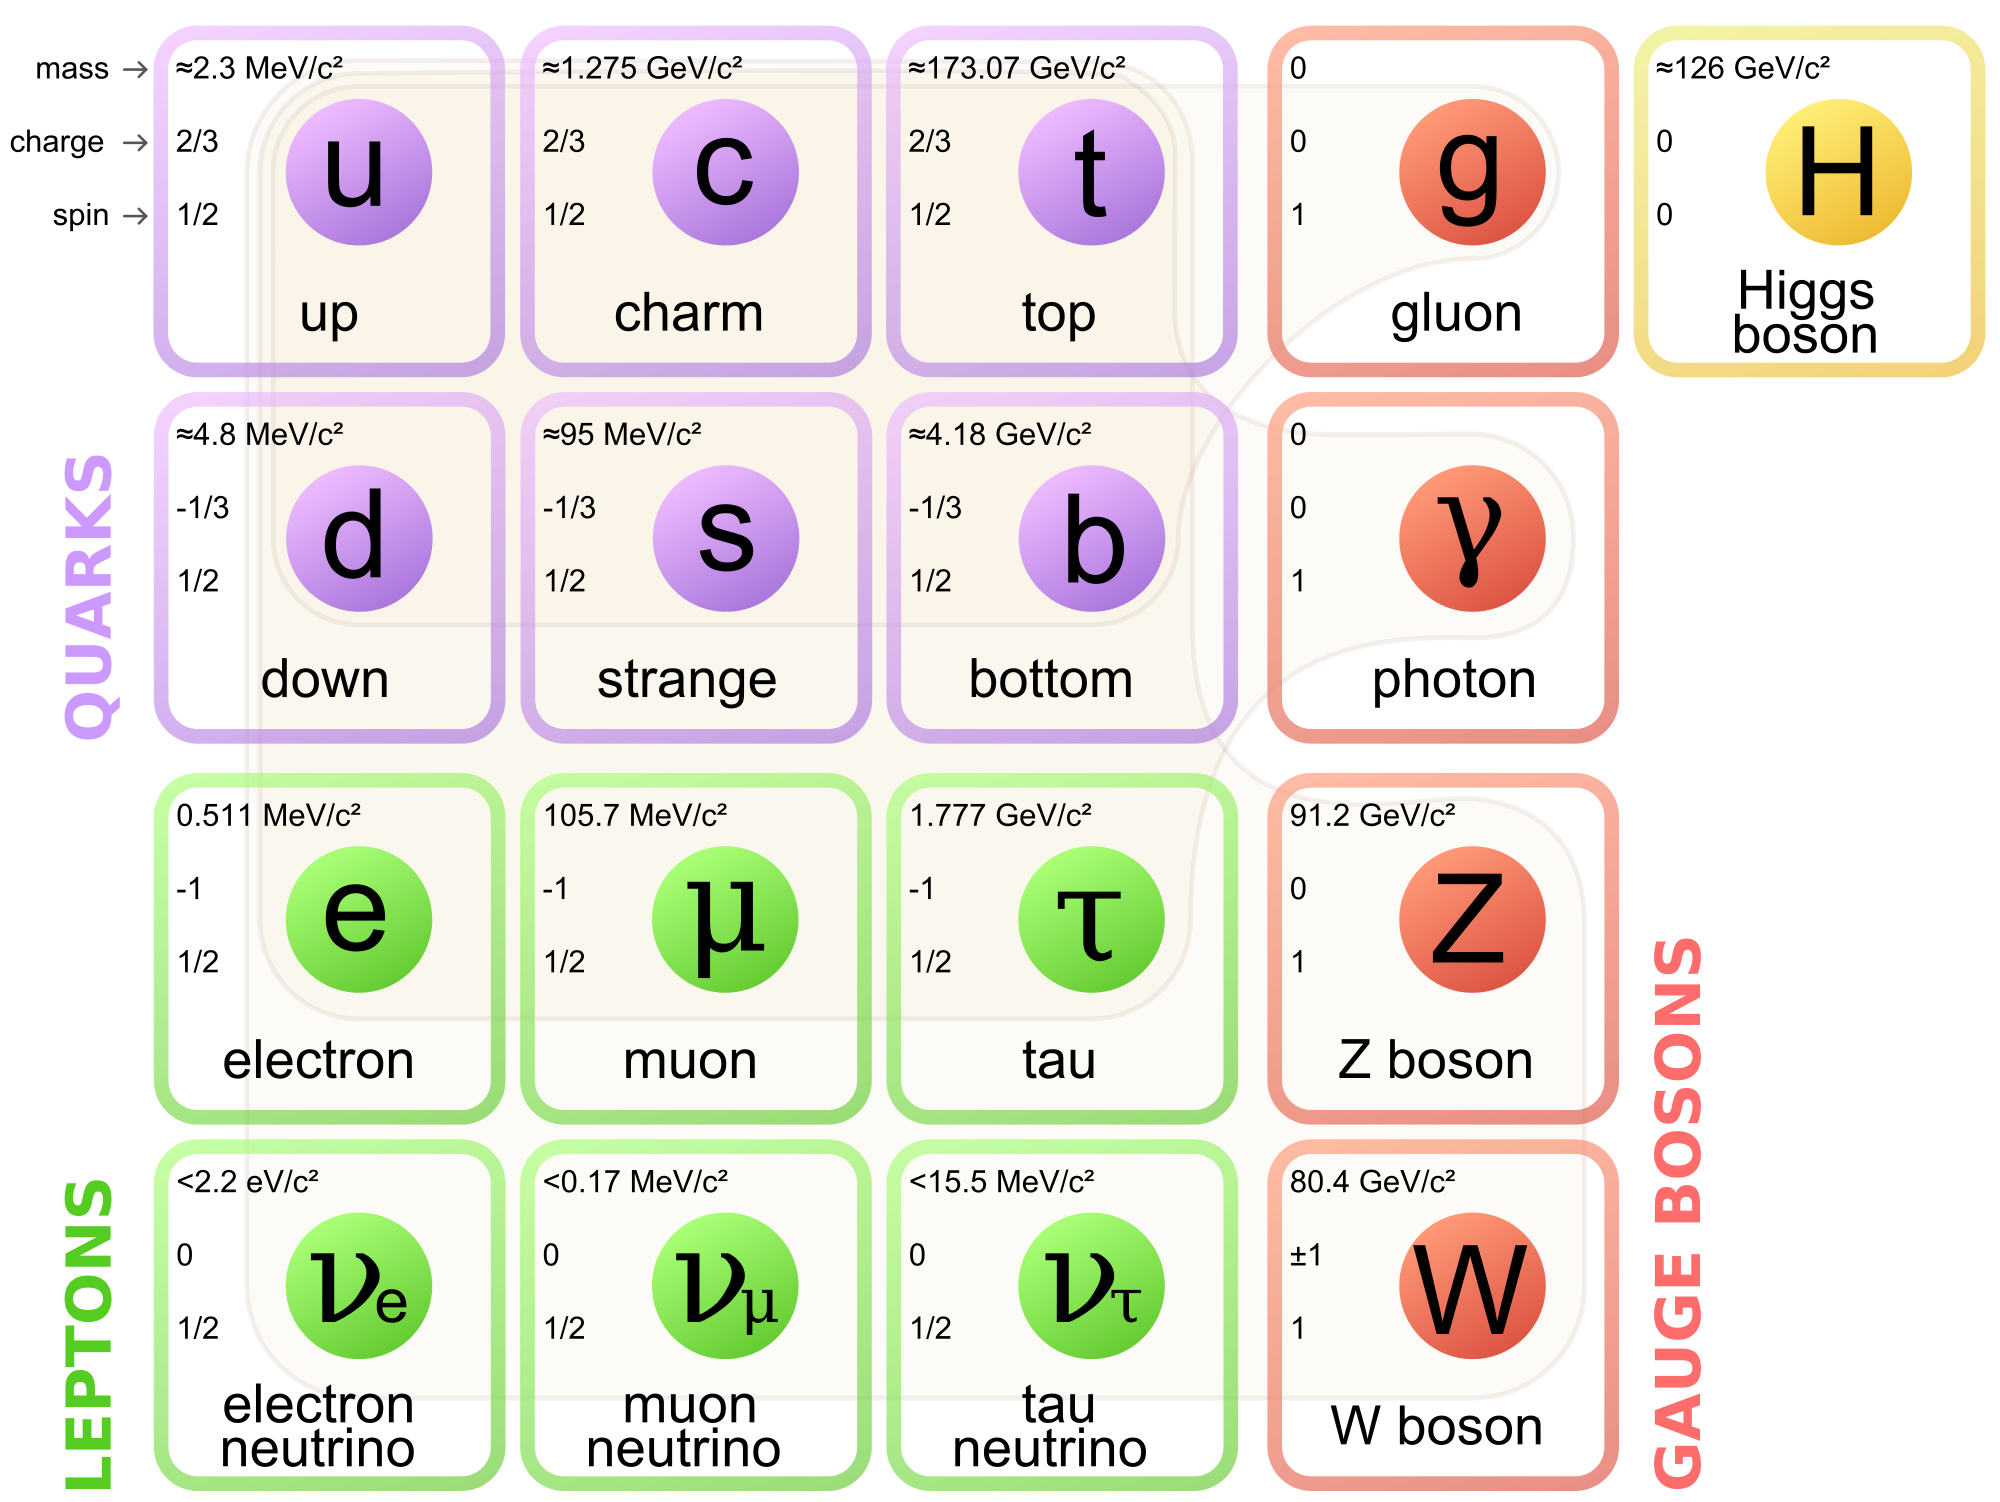
\includegraphics[width=0.6\textwidth]{01_Theory_SM/plots/Standard_Model_of_Elementary_Particles.png}
  \caption{The Standard Model of Elementary Particle Physics with three generations of matter fermions, field bosons and a Higgs boson. 
  The properties of the particles are also shown in each box.}
  \label{fig:SM_Particles}
\end{figure}


\subsection{Leptons}

The two bottom rows of fermions at the Fig.\ref{fig:SM_Particles} represent the known \textit{leptons} with their masses, charges
and spins. 

In general, the fermions are described with the Dirac equation\cite{diraceq}:

\begin{equation}\label{eq:dirac}
  i\hbar\gamma^{\mu}\partial_{\mu}\psi - mc\psi = 0 ,
\end{equation}

where the $\psi$ is a four-element Dirac spinor, an equivalent of a one dimentional Schr\"{o}dinger wave function, 
$\gamma^{\mu}$s are the gamma matricies and $\partial_{\mu}$ is a partial derivative with respect to the time-space four-vector
components. 

Dirac equation \ref{eq:dirac} has solutions with positive but also with negative energy states. Those are treated
as \textit{antiparticles}. So every lepton, being a fermion, has an antiparticle. At the Fig.\ref{fig:SM_Particles}
only particles are shown. Electron $e^{-}$ has an antiparticle positron $e^{+}$. The muon $\mu^{-}$, tau $\tau^{-}$ and
their antiparticles, $\mu^{+}$ and $\tau^{+}$ differ from the electron and positron only by their masses and their lifetimes.

Neutral leptons, neutrinos $\nu$, also have antiparticles, antineutrinos $\bar{\nu}$. Every massive lepton has a corresponding
neutrino: $\nu_{e}$, $\nu_{\mu}$ and $\nu_{\tau}$. It is believed that in the interactions a lepton can change only to another
of this type. This is known as \textit{conservation of lepton number}. In this rule leptons have positive lepton numbers and
antileptons -- negative ones.

\subsection{Quarks}

The upper two rows 

% \section{Interaction}
% \subsection{Bosons}
% \subsection{Electrmagnetic Interaction}
% \subsection{Strong Interaction}
% \subsection{Weak Interaction and Electroweak Symmetry Breaking}
% \subsection{Gravitation}
% 
% \section{Top Physics}
% \subsection{Top Quark Production}
% \subsection{Top Quark Decay}
% \section{Deep Inelastic Scattering at HERA}
